% !TEX program = pdflatex
% TeXora sample lecture. Everything here is neutral placeholder text: replace it with your own.
% TeXora sample lecture, edition 2
\documentclass[aspectratio=43]{beamer}
\usetheme{Madrid}
\useoutertheme[subsection=false]{miniframes}
\usepackage{amsmath,amssymb,tikz}
\usetikzlibrary{arrows.meta,positioning}
\tikzset{visible on/.style={alt={#1{}{opacity=0,text opacity=0}}},alt/.code args={<#1>#2#3}{\alt<#1>{\pgfkeysalso{#2}}{\pgfkeysalso{#3}}}}
\definecolor{leaf}{RGB}{74,132,58}
\definecolor{leafdark}{RGB}{33,65,29}
\setbeamercolor{structure}{fg=leaf}
\setbeamercolor{palette primary}{bg=leafdark,fg=white}
\setbeamercolor{palette secondary}{bg=leafdark!80!leaf,fg=white}
\setbeamercolor{palette tertiary}{bg=leaf,fg=white}
\setbeamercolor{palette quaternary}{bg=leafdark,fg=white}
\setbeamercolor{title}{bg=leaf,fg=white}
\setbeamercolor{frametitle}{bg=leaf,fg=white}
\setbeamercolor{section in head/foot}{bg=leafdark,fg=white}
\setbeamercolor{block title}{bg=leaf,fg=white}
\setbeamercolor{block body}{bg=leaf!10}
\setbeamertemplate{blocks}[rounded][shadow=true]
\setbeamertemplate{section in toc}[ball]
\setbeamertemplate{bibliography item}[text]
\setbeamerfont{note page}{size=\small}
\setbeameroption{show notes on second screen=right}

\title[Graph Search in Practice]{A Sample Lecture on Graph Search}
\subtitle{From Textbook Pseudocode to Reproducible Experiments}
\author[Your Name]{Your Name}
\institute[Your University]{Your University}
\date[Sample Seminar]{Research Seminar \\[1em] 2026}

\begin{document}

\begin{frame}
  \titlepage
  \note{Hi everyone. \textbf{Thanks for being here.} Today I am walking through a sample lecture on graph search.\\
  We will explore where the classic algorithms come from and what they mean for real workloads.\\
  The big idea is: if we want results people can trust, we need structure, not just speed.\\
  Before diving in, let me quickly outline what we will cover today.}
\end{frame}

\begin{frame}{Content}
  \tableofcontents
  \note{Six parts. Spend most of the time on the approach and the evaluation.\\
  Skip the foundations if the audience already knows BFS.}
\end{frame}

\section{Introduction}
\begin{frame}{Why Graph Search Still Matters}
  \begin{itemize}
    \item<1-> Road networks, citation graphs and dependency trees
    \item<2-> Small changes to the frontier change the whole cost
    \item<3-> Reproducing a published result is harder than it looks
  \end{itemize}
  \note{Reveal one bullet at a time. Ask who has tried to reproduce a benchmark.
    \begin{itemize}
      \item Road networks: mention the city map example
      \item \textbf{Pause} before the last point
    \end{itemize}}
\end{frame}

\begin{frame}{Research Questions}
  \begin{block}<1->{RQ1}Which frontier gives the best trade-off on sparse graphs?\end{block}
  \begin{block}<2->{RQ2}How stable are the results across hardware?\end{block}
  \note{Both questions are answered in the evaluation section. Point forward to the summary table.}
\end{frame}

\section{Related Work}
\begin{frame}{A Short History}
  \begin{itemize}
    \item Shortest paths with a priority queue~\cite{dijkstra}
    \item Heuristic search with admissible estimates~\cite{hart}
    \item Community benchmarks for reproducibility~\cite{bench}
  \end{itemize}
  \note{The citations are links. In TeXora, hover one to peek at the reference without leaving this slide.}
\end{frame}

\section{Approach}
\begin{frame}{The Core Recurrence}
  \begin{equation*}
    d(v) \;=\; \min_{(u,v)\in E}\bigl( d(u) + w(u,v) \bigr)
  \end{equation*}
  \pause
  \begin{equation*}
    f(v) \;=\; d(v) + h(v), \qquad h(v) \le d^\ast(v)
  \end{equation*}
  \note{First the plain recurrence, then add the heuristic.\\ Stress that the estimate must never overshoot.}
\end{frame}

\begin{frame}{Search Pipeline}
  \centering
  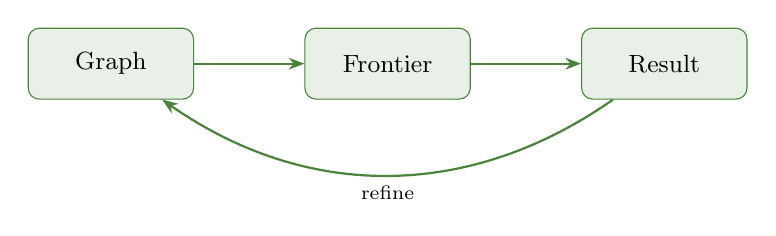
\begin{tikzpicture}[node distance=1.1cm and 1.4cm, box/.style={draw=leaf,fill=leaf!12,rounded corners,minimum width=2.1cm,minimum height=.9cm,font=\small}, >={Stealth[length=2mm]}]
    \node[box] (a) {Graph};
    \node[box,right=of a,visible on=<2->] (b) {Frontier};
    \node[box,right=of b,visible on=<3->] (c) {Result};
    \draw[->,thick,leaf,visible on=<2->] (a) -- (b);
    \draw[->,thick,leaf,visible on=<3->] (b) -- (c);
    \draw[->,thick,leaf,visible on=<3->] (c) to[bend left=35] node[below,font=\scriptsize,text=black]{refine} (a);
  \end{tikzpicture}
  \note{Build the diagram step by step. The loop back is the part people forget.}
\end{frame}

\begin{frame}{Worked Example}
  \begin{enumerate}
    \item<1-> Start from the source with distance zero
    \item<2-> Relax each outgoing edge
    \item<3-> Pop the smallest tentative distance
    \item<4-> Repeat until the target is settled
  \end{enumerate}
  \note{Use the pen to trace the order on the board. Use the laser to point at step three.}
\end{frame}

\section{Foundations}
\begin{frame}{Complexity at a Glance}
  \centering
  \begin{tabular}{lll}
    \textbf{Method} & \textbf{Time} & \textbf{Space}\\\hline
    Breadth-first & $O(V+E)$ & $O(V)$\\
    Binary heap & $O(E\log V)$ & $O(V)$\\
    Fibonacci heap & $O(E+V\log V)$ & $O(V)$
  \end{tabular}
  \note{Mention that the theoretical winner is rarely the practical winner.}
\end{frame}

\section{Evaluation}
\begin{frame}{Experimental Setup}
  \begin{itemize}
    \item Twelve sparse graphs, three dense graphs
    \item Five repetitions, median reported
    \item Fixed seeds and pinned library versions
  \end{itemize}
  \note{Keep this short. Details are in the backup slide if someone asks.\\ \hyperlink{backup-setup}{Backup: full setup.}}
\end{frame}

\begin{frame}{Sample Results}
  \centering
  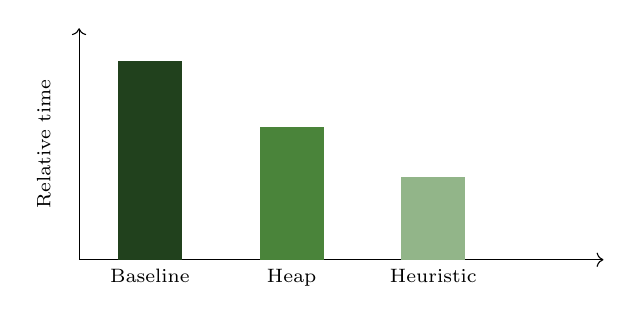
\begin{tikzpicture}[x=.9cm,y=.42cm]
    \draw[->] (0,0) -- (7.4,0); \draw[->] (0,0) -- (0,7);
    \foreach \x/\h/\c in {1/6/leafdark,3/4/leaf,5/2.5/leaf!60}
      \fill[\c] (\x-.45,0) rectangle (\x+.45,\h);
    \node[below,font=\scriptsize] at (1,0) {Baseline};
    \node[below,font=\scriptsize] at (3,0) {Heap};
    \node[below,font=\scriptsize] at (5,0) {Heuristic};
    \node[rotate=90,font=\scriptsize] at (-.5,3.5) {Relative time};
  \end{tikzpicture}
  \note{These numbers are invented placeholders for the demo. The takeaway: the heuristic halves the runtime.}
\end{frame}

\section{Conclusion}
\begin{frame}{Take-Home Messages}
  \begin{enumerate}
    \item Choose the frontier for your graph, not for the textbook
    \item Publish seeds, versions and raw data
    \item Questions welcome
  \end{enumerate}
  \note{Pause here. Leave this slide up during the questions.}
\end{frame}

\appendix
\section*{Backup}
\begin{frame}[label=backup-setup]{Backup: Full Setup}
  \small
  \begin{itemize}
    \item Sixteen cores, 64 GB of memory
    \item Compiler optimisation level three
    \item Timings exclude graph loading
  \end{itemize}
  \note{Only show this if someone asks about the hardware.}
\end{frame}

\begin{frame}{References}
  \footnotesize
  \begin{thebibliography}{9}
    \bibitem{dijkstra} E. W. Dijkstra. A note on two problems in connexion with graphs. \emph{Numerische Mathematik}, 1959.
    \bibitem{hart} P. E. Hart, N. J. Nilsson and B. Raphael. A formal basis for the heuristic determination of minimum cost paths. \emph{IEEE Trans. SSC}, 1968.
    \bibitem{bench} Placeholder Authors. Sample benchmark collection. \emph{Example Proceedings}, 2020.
  \end{thebibliography}
  \note{Reference slide. Reached from the citation links.}
\end{frame}
\end{document}
